%\documentclass[12pt]{scrartcl}
\documentclass[12pt]{article}
\usepackage{amsmath}
\usepackage{amsfonts}
\usepackage{amsthm}
\usepackage{amssymb}
\usepackage{bbm}
\usepackage[hidelinks]{hyperref}
\usepackage{color}
\usepackage{graphicx}
%\usepackage[export]{adjustbox}
\usepackage{float}
\usepackage{caption}
\captionsetup{font=footnotesize}

\usepackage{easy-todo}

\DeclareMathOperator{\di}{d\!}
\newcommand*\Eval[3]{\left.#1\right\rvert_{#2}^{#3}}

%\usepackage[backend=biber,style=apa]{biblatex}
%\DeclareLanguageMapping{british}{british-apa}
%\usepackage{epigraph}
%\usepackage{dsfont}
\usepackage{setspace}
\usepackage{cleveref}
\usepackage{natbib}
\usepackage{etoolbox}
\usepackage[margin=0.7in]{geometry}
%\setlength{\epigraphwidth}{5.5in}
\usepackage{accents}
\usepackage{lscape}
\usepackage[normalem]{ulem}
\useunder{\uline}{\ul}{}

\newcommand{\ubar}[1]{\underaccent{\bar}{#1}}
\newcommand\addtag{\refstepcounter{equation}\tag{\theequation}}

\newtheorem{prop}{Proposition}
\newtheorem{lemm}{Lemma}
\newtheorem{thm}{Theorem}
\newtheorem{conj}{Conjecture}
\newtheorem{assn}{Assumption}
\newtheorem{defn}{Definition}
\newtheorem{coro}{Corollary}


\title{Calibrating the model}

\author{Akhil Rao, Matthew Burgess, Daniel Kaffine}

\begin{document}
	
	\maketitle

\section{Calibrating the physical model}	

Our model uses the accounting relationships in the aggregate stocks of satellites and debris for the laws of motion, and draws on \cite{bradleywein2009} for the functional forms of the new fragment creation and collision rate functions. The scale of the time period is taken as one year, but can be shortened or lengthened by adjusting the discount rate and profits per satellite. $S_t$ denotes the number of active satellites in an orbital shell in period $t$, $D_t$ the number of debris objects in the shell in $t$, $X_t$ the number of satellites launched in $t$, $\ell_t$ the probability that an active satellite in the shell will be destroyed in a collision in $t$, $Z_t$ is the fraction of satellites which deorbit in $t$, and $\mu$ is the average amount of debris generated by deorbiting satellites. $\delta$ is the average proportion of debris objects which deorbit in $t$, and $G(S_t,D_t,\ell_t)$ is the number of new debris fragments generated due to all collisions between satellites and debris. $m$ is the number of debris pieces contributed by satellites launched. $A_t$ is the number of anti-satellite missile tests conducted in $t$, and $\gamma_A$ is the average number of fragments created by one test. $L_t$ is the number of satellites actually destroyed in collisions with other satellites or debris. \footnote{For most of our sample, $L_t$ is zero. We use $\ell_t$ rather than $L_t$ in equation \ref{debrisLoM} because the ECOB risk index which we use to measure $\ell_t$ proxies for unobserved collisions, including non-catastrophic ones. Second, as the number of objects and time horizon increase, the fraction of satellites destroyed in collisions converges to the probability an active satellite is destroyed in a collision.}\\

The number of active satellites in orbit is modeled as the number of launches in the previous period plus the number of satellites which survived the previous period. The amount of debris in orbit is the amount from the previous period which did not decay, plus the number of new fragments created in collisions, plus the amount of debris in the shell created by new launches. Formally,
\begin{align}
\label{satelliteLoM}
S_{t+1} &= S_t -L_t -Z_tS_t + X_t \\
\label{debrisLoM}
D_{t+1} &= D_t(1-\delta) + \mu Z_tS_t + mX_t + G(S_t,D_t,\ell_t) + \gamma_A A_t.
\end{align}

\cite{bradleywein2009} use an ideal gas model to parameterize $G(S_t,D_t,\ell_t)$ as a quadratic function of the number of objects in orbit. We therefore approximate it as
\begin{equation}
\label{growthFunction}
G(S_t,D_t,\ell_t) = \beta_{SS} \left( \frac{S_t}{S_t+D_t} \right ) \ell_t S_t + \beta_{SD}\left( \frac{D_t}{S_t+D_t} \right ) \ell_t S_t +  \beta_{DD} \alpha_{DD} D_t^2,
\end{equation}

where the $\alpha_{jk}$ parameters are intrinsic collision probabilities between objects of type $j$ and $k$, and $\beta_{jk}$ parameters are effective numbers of fragments from such collisions\footnote{``Intrinsic collision probabilities'' measure the probability that two objects of given sizes moving randomly in a box of fixed volume will collide in a unit of time. ``Effective numbers of fragments'' measure the number of new fragments weighted by the time they spend inside the volume of interest.}. Similarly, we parameterize $\ell_t$ as

\begin{equation}
\label{collFunction}
\ell_t = \alpha_{SS} S_t^2 + \alpha_{SD} S_t D_t
\end{equation}

where $\alpha_{SS}$ and $\alpha_{SD}$ intrinsic collision probabilities of satellite-satellite and between satellites-debris collisions. We refer to the intrinsic collision probabilities and effective numbers of fragments as \textit{structural physics parameters}. Equations \ref{debrisLoM}, \ref{growthFunction}, and \ref{collFunction} can be viewed as reduced-form statistical models which recreate the results of higher-fidelity physics-based models of debris growth and the collision rate

\subsection*{Data}

We use data on satellites in orbit from the Space-Track dataset hosted by the Combined Space Operations Center (CSpOC) \citep{spacetrackData} to construct the satellite stock and launch rate series'. The Space-Track dataset provides details on active payloads in LEO and their decay dates. We construct the launch rate as

\begin{equation}
X_t = S_{t+1} - S_t - Z_tS_t,
\end{equation}

where $S_t$ is the number of active payloads in year $t$ and $Z_tS_t$ is the number of payloads listed as decayed in year $t$. \\

The debris and collision risk series' we use were provided by the European Space Agency. We use debris data from the DISCOS database \citep{FRAGdata} and collision risk index data provided by Dr. Francesca Letizia \citep{ECOBdata}. We use only objects with a semi-major axis of 2000km or less in all our data series. We prefer to use the DISCOS fragment data rather than the Space-Track fragment data as it tracks fragments from the time they were created or detected, whereas the Space-Track data tracks fragments from the time their parent body was launched. The DISCOS attribution method is closer to how economic agents in our model receive information and make decisions. We record the number of anti-satellite missile tests in a year using data from Wikipedia \citep{ASATdata}.

\todoi{Distinguish between expected collision rate and realized destructions}

\subsection*{Calibration procedure}
We calibrate equations \ref{collFunction} and \ref{debrisLoM} by estimating the following equations:
\begin{align}
\label{riskEstimation}
E_{t-1}[\ell_t|S_t,D_t] &= a_{\ell 1} S_t^2 + a_{\ell 2} S_t D_t + \epsilon_{\ell t}  \\
\label{debLoMEstimation}
D_{t+1} &= a_{D 1} D_t + a_{D 2}Z_tS_t + a_{D 3} X_t  + a_{D4} \left( \frac{S_t}{S_t+D_t} \right ) \ell_t S_t + a_{D5}\left( \frac{D_t}{S_t+D_t} \right ) \ell_t S_t + \\
&~~  a_{D6} D_t^2 + a_{D7}A_t + \epsilon_{D t},
\end{align}

where $\epsilon_{xt}$ are mean-zero error terms to minimize and $a_{xi}$ are parameters to estimate. All $a_{xi}$ are nonnegative in theory, with $a_{S1}$ and $a_{D1}$ being in $(0,1)$. The correspondence between $a_{xi}$ and the structural physics parameters is shown below:
\begin{align*}
a_{\ell 1} &= \alpha_{SS}, ~~ a_{\ell 2} = \alpha_{SD} \\
a_{D1} &= 1-\delta, ~~ a_{D 2} = \mu, ~~ a_{D 3} = m, ~~ a_{D4} = \beta_{SS}, ~~ a_{D5} = \beta_{SD}, ~~ a_{D6} = \beta_{DD}\alpha_{DD}, ~~ a_{D7} = \gamma_A
\end{align*}

$\beta_{DD}$ and $\alpha_{DD}$ are not separately identified from these regressions. \\

We estimate equation \ref{riskEstimation} using OLS on the full sample, and equation \ref{debLoMEstimation} using ridge regression on a quarter of the sample, evenly spaced. The fitted values are shown against the actual values with residuals in figure \ref{debCalibration}. We report a sensitivity analysis of our sampling procedure for equation \ref{debLoMEstimation} in the Appendix.

\begin{figure}[H]
	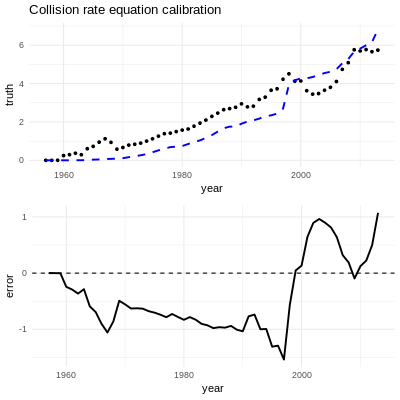
\includegraphics[width=0.5\textwidth]{../../images/risk_fit_plot.png}
	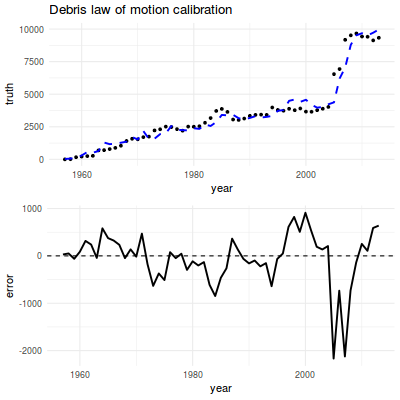
\includegraphics[width=0.5\textwidth]{../../images/debris_lom_fit_plot.png}
	\captionsetup{format=hang}
	\caption{\textit{Calibration fit.} \\
		The upper panels show fitted values (blue dashed line) against actual values (black dots). The lower panels show the residuals.
	}
	\label{debCalibration}
\end{figure}

Tables \ref{riskParms} and \ref{debParms} show the calibrated parameters:

\begin{table}[H]
	\centering
	\begin{tabular}{|l|l|l|}
		\hline
		\textit{Expected collision risk parameters:}      & \textbf{$\alpha_{SS}$} & \textbf{$\alpha_{SD}$} \\ \hline
		\textit{Parameter values:} & 1.15e-09               & 9.49e-11               \\ \hline
		\textit{Standard errors:} & 7.71e-11 & 2.2e-11 \\ \hline
	\end{tabular}
	\caption{Parameter values from estimating equation \ref{riskEstimation}.}
	\label{riskParms}
\end{table}

\begin{table}[H]
	\begin{tabular}{|l|l|l|l|l|l|l|l|}
		\hline
		\textit{Debris law of motion parameters} & \textbf{$\delta$} & \textbf{$\mu$} & \textbf{$m$} & \textbf{$\gamma_A$} & \textbf{$\beta_{SS}$} & \textbf{$\beta_{SD}$} & \textbf{$\beta_{DD}\alpha_{DD}$} \\ \hline
		\textit{Parameter values:}                           & 0.52              & 5.83           & 2.19         & 604.04              & 336.42                & 127.96                & 2.1e-05                          \\ \hline
	\end{tabular}
		\caption{Parameter values from estimating equation \ref{debLoMEstimation}. All values except $\beta_{DD}\alpha_{DD}$ are rounded to two decimal places. Standard errors are not reported due to the estimation bias in ridge regression.}
		\label{debParms}
\end{table}

These parameter values are physically plausible, with the values estimated for equation \ref{debLoMEstimation} being lower bounds\footnote{Ridge estimates are biased toward zero relative to OLS estimates. For a given penalty parameter $\lambda \geq 0$, the relationship between a ridge coefficient estimate $\hat{\beta}^{\text{ridge}}$ and the corresponding OLS estimate $\hat{\beta}^{\text{OLS}}$ is $\hat{\beta}^{\text{ridge}} = \hat{\beta}^{\text{OLS}}/(1+\lambda)$.}. For example, the value of $m$ suggests that every satellite launched creates $2.19$ pieces of debris on average, while the value of $\gamma_A$ suggests that anti-satellite missile tests create $604.04$ pieces of debris on average. While the true number is likely to be higher, the orders of magnitude between $\gamma_A$, $\beta_{SS}$, and $\beta_{SD}$ seem reasonable: firing a missile at a satellite creates the most debris due to the explosives involved, collisions between two satellites creates an intermediate amount of debris, and collisions between a satellite and  a debris fragment create the least amount of debris in part because there is the least amount of mass to be fragmented. The expected amount of debris created by debris-debris collisions is $2e-05$ fragments - a small number, but plausible considering that fragments are small and (a) unlikely to collide, and (b) have less mass to be fragmented when they do collide.

\section*{Calibrating the economic model}

Our economic model draws on \cite{raorondinaWP} to determine the satellite launch rate, $X_t$, as a function of the collision risk, $\ell_{t+1}$, and the excess return on a satellite, $r_{s} - r$. In the simplest case, where all of the economic parameters are constant over time, the launch rate solves
\begin{equation}
\label{OAeqm}
E_t[\ell_{t+1}|S_{t+1},D_{t+1}] = r_s - r,
\end{equation}

where $r_s$ is the per-period rate of return on a single satellite ($\pi/F$, where $\pi$ is the per-period return generated by a satellite and $F$ is the cost of launching a satellite, inclusive of non-launch expenditures such as satellite manufacturing and ground stations) and $r$ is the risk-free interest rate. In general, the open access launch rate equates the expected collision rate in period $t+1$, given information in period $t$, with the expected rate of excess return in period $t+1$. More precisely, $r$ is the opportunity cost of funds invested in launching a satellite, and may diverge from the risk-free rate if the satellite launcher's most-preferred alternate investment is not a risk-free security. This rate is sometimes referred to as the internal rate of return (IRR). Equation \ref{OAeqm} can therefore also be used to calculate the implied IRR for satellite investments from observed data on collision risk and satellite returns. $r$ is not observed in our data. When costs, returns, and the discount rate are all time-varying, equation \ref{OAeqm} becomes
\begin{equation}
\label{OAeqm2}
E_t[\ell_{t+1}|S_{t+1},D_{t+1}] = 1+ r_{s,t+1} - (1+r_t) \frac{F_t}{F_{t+1}},
\end{equation}

where $r_{s,t+1} = \pi_{t+1}/F_{t+1}$. The first term, $1+r_{s,t+1}$, is the gross return on a single satellite in period $t+1$. The second term, $(1+r_t) \frac{F_t}{F_{t+1}}$, is the gross return on the firm's alternate investment had they invested in period $t$.

\subsection*{Data}

We use data on satellite industry revenues from \citet{wienzierl2018}, and data on satellites in LEO (semi-major axis less than 2000km) from the Union of Concerned Scientists' list of active satellites \citep{UCSdata}. The economic data provide a breakdown of revenues across satellite manufacture, launch, insurance, and products and services. The satellite industry revenues data cover 2005-2015, while the active satellites data cover 1958-2017. \\

We calculate the per-period returns on owning a satellite ($\pi_t$) as the revenues generated from commercial space products and services, and the per-period costs of launching a satellite ($F_t$) as the sum of revenues from commercial infrastructure and support industries, ground stations and equipment, commercial satellite manufacturing, and commercial satellite launching. The ratio $\pi_t/F_t$ then gives a time series of the rate of return on a single satellite, as the number of satellites cancels out of the numerator and denominator. Since the numbers provided in \citet{wienzierl2018} are for the satellite industry as a whole, the ratio still needs to be adjusted to represent satellites in LEO. We adjust for this by calculating the yearly share of satellites in LEO and multiplying the ratio by this share. \\

\subsection*{Calibration procedure}

Since the IRR is unobserved, we calibrate equation \ref{OAeqm2} by estimating
\begin{equation}
\ell_{t} = a_{\ell 1} + a_{\ell 2} r_{st} + a_{\ell 3} \frac{F_{t-1}}{F_t} + \epsilon_{r t},
\end{equation}

using OLS on the full sample\footnote{We omit the first observation, for 2005, to construct $F_{t-1}/F_{t}$.}, where $\epsilon_{rt}$ is a mean-zero error term, $a_{\ell 2}$ is a scale parameter, and $a_{\ell 3}$ measures the gross IRR, $1+r$. The fitted values are shown against the actual values with residuals in figure \ref{econCalibration}.

\begin{figure}[H]
	\centering
	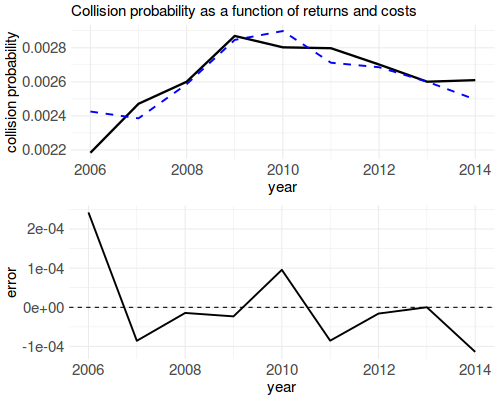
\includegraphics[width=0.5\textwidth]{../../images/risk_return_plot.png}
	\captionsetup{format=hang}
	\caption{\textit{Calibration fit.} \\
		The upper panel shows fitted values (blue dashed line) against actual values (black solid line). The lower panel shows the residuals.
	}
	\label{econCalibration}
\end{figure}

Tables \ref{econParms} shows the calibrated parameters:

\begin{table}[H]
	\centering
	\begin{tabular}{|l|l|l|l|}
		\hline
		\textit{Economic calibration parameters:}      & \textbf{$a_{\ell 1}$} & \textbf{$a_{\ell 2}$} & \textbf{$a_{\ell 3}$} \\ \hline
		\textit{Parameter values:} & 0.004               & 0.009               & - 0.0004 \\ \hline
		\textit{Standard errors:} & 0.002 & 0.002 & 0.001 \\ \hline
	\end{tabular}
	\caption{Parameter values from estimating equation \ref{OAeqm2}. All values are rounded to the first non-zero digit.}
	\label{econParms}
\end{table}

If our data perfectly measured the costs and returns of satellite ownership, and our theoretical model held exactly, we would expect $a_{\ell 1}=1$, $a_{\ell 2} = 1$, and $a_{\ell 3} < -1$. Instead, we estimate $a_{\ell 1}=0.004$, $a_{\ell 2} = 0.009$, and $a_{\ell 3} = -0.0004$. This suggests that our returns and cost series are measured with error or that our theoretical model is missing some important factors, such as constraints on the number of launches possible each period. \\

\subsubsection*{Measurement error}

Random measurement error would attenuate coefficient estimates, which may partially explain why our estimated coefficients are close to zero. Non-random measurement error is another possibility. \\

We construct the returns and costs of satellite ownership from the data described in \citet{wienzierl2018}, which aggregate revenues from all commercial satellites in orbit. Our physical model is based on data for low Earth orbit. To adjust the returns and costs to reflect only satellites in LEO, we multiply the per-period returns and cost series' by the share of satellites launched each year to LEO. If the returns to LEO satellites are lower than the returns to GEO satellites, then our attribution procedure would overstate the returns to LEO. The near-zero coefficients may therefore partially reflect systematically overstated returns to LEO in our constructed series'.

\subsubsection*{Launch constraints}

Our theoretical model assumes that any firm which wants to launch a satellite can do so. If launches are limited, they will be unable to do so. This will prevent open access launching from equating the excess return on a satellite with the risk of its destruction. Firms which are able to launch will then earn rents from having a satellite while the collision risk is below the excess return. The wedge between the collision risk and excess return will reflect the value of those rents. \\

Launch limitations which allow only $\bar{X}_t$ firms to launch in $t$ are a type of ``flow control'', studied in more depth in \citet{raoJMP}. In particular, \citet{raoJMP} establishes that flow controls which restrict the quantity of launches in each period are equivalent to flow controls which impose an additional positive price $p_t$ on launching in $t$. Generalizing the flow-controlled equilibrium condition from that paper, we obtain the open access equilibrium condition for launches when costs, returns, and discount rates are all time-varying:

\begin{equation}
\label{OAfloweqmcond}
\ell_{t+1} = (1 - \frac{p_t}{F_{t+1} + p_{t+1}}) + \frac{\pi_{t+1}}{F_{t+1} + p_{t+1}} - (1+r_t)\frac{F_t}{F_{t+1} + p_{t+1}},
\end{equation}

$p_t$ can be interpreted in two ways. It may be viewed as the implied rent received by a firm which already owns a satellite in $t$ due to launches in $t$ being restricted. It may also be viewed as the implied launch tax paid by a firm which is allotted a launch slot in $t$. In either view, a binding launch constraint results in positive values of $p_t$ and $p_{t+1}$, biasing the coefficients from regression \ref{OAeqm2} downwards. %toward negative infinity ($a_{\ell 1}$) or zero ($a_{\ell 2}$ and $a_{\ell 3}$).

\newpage

{
	\setlength{\bibsep}{3pt}
	\setstretch{1}
	\bibliography{../database}
	\bibliographystyle{jpe}
}

\newpage
\section*{Appendix}

\subsection*{Sensitivity analysis of sampling procedure for estimating equation \ref{debLoMEstimation}}

We estimate equation \ref{debLoMEstimation} using only a quarter of the sample to avoid overfitting. To evaluate how sensitive the predictions and coefficient estimates are to our sampling procedure, we conduct a sensitivity analysis. Our procedure is straightforward. We randomly draw a quarter of the sample (15 observations) 1000 times, estimate equation \ref{debLoMEstimation} on each random sample, and plot the predictions against the observed $D_{t+1}$ in figure \ref{debSensitivityFig}. We also take the mean of the estimated coefficients and compare them against the model we selected in table \ref{debParms}. Table \ref{debSensitivityCoefs} shows the comparison.

\begin{figure}[H]
	\centering
	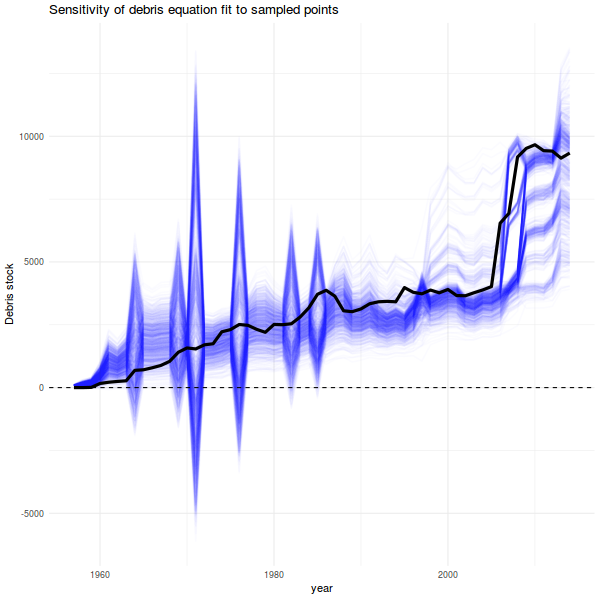
\includegraphics[width=0.7\textwidth]{../../images/debris_lom_sensitivity_plot.png}
	\captionsetup{format=hang}
	\caption{\textit{Calibration fit.} \\
		The thin blue lines show fits from random samples. The thick black line shows the actual debris time series. The large sometimes-negative spikes in the predicted series' correspond to anti-satellite missile tests, of which the 2007 FY-1C test generated the most debris.
	}
	\label{debSensitivityFig}
\end{figure}

\begin{table}[H]
	\begin{tabular}{|l|l|l|l|l|l|l|l|l|}
		\hline
		\textit{Debris law of motion parameters} & \textbf{$\delta$} & \textbf{$\mu$} & \textbf{$m$} & \textbf{$\gamma_A$} & \textbf{$\beta_{SS}$} & \textbf{$\beta_{SD}$} & \textbf{$\beta_{DD}\alpha_{DD}$} & $\lambda$ \\ \hline
		\textit{Model selected in table \ref{debParms}:}                           & 0.52              & 5.83           & 2.19         & 604.04              & 336.42                & 127.96                & 2.1e-05  &    287.21                     \\ \hline
		\textit{Mean parameter values:}                           & 0.76              & 16.19           & 2.31         & 156.57              &  487.68                & 137.94                & 1.9e-05      &  325.61                  \\ \hline
	\end{tabular}
	\caption{Parameter values from estimating equation \ref{debLoMEstimation}. All values except $\beta_{DD}\alpha_{DD}$ are rounded to two decimal places. $\lambda$ is the ridge penalty parameter, with larger values corresponding to greater shrinkage (and coefficient bias). We selected $\lambda$ by cross-validation on the training sample in all cases.}
	\label{debSensitivityCoefs}
\end{table}

\end{document}
